\documentclass{article}
\usepackage{graphicx}
\usepackage{amsmath}

\AddToHook{cmd/section/before}{\clearpage}

\title{\textbf{CS 194: Keshav's First Pass}}

\author{
    CASTRO, Raniel Emil C.
    \and
    DOMINGO, Karlo S.
    \and
    EUSEBIO, Azrael Darius O.
    \and
    PILAPIL, Marcus Corso S.
    \and
    (Group Name: \textit{93})
    }

\date{\textit{\today}}

\begin{document}

\maketitle

\section{A Mathematical Theory of Communication (2)}

\begin{enumerate}
    \item \textit{Category:} This paper is a theoretical paper in the field of communication. It tackles the problem of 
    communication through a mathematical procedure and fundamental concepts of communication.
    
    \item \textit{Context:} This paper is an extension of the papers of Nyquist and Hartley about the general theory of
    communication. It includes newer factors like the effect of noise in the channel and statistical
    structure savings possible. It uses mathematical theories and statistical analysis.

    Nyquist, H., “Certain Factors Affecting Telegraph Speed,” \textit{Bell System Technical Journal}, April
    1924, p. 324; “Certain Topics in Telegraph Transmission Theory,” \textit{A.I.E.E. Trans.}, v. 47, April
    1928, p. 617.

    Hartley, R. V. L., “Transmission of Information,” \textit{Bell System Technical Journal}, July 1928, p. 535.

    \item \textit{Correctness:} Assumptions appear to be valid. The paper shows a lot of mathematical and statistical
    procedures including approximations, models, graphs, entropy, and decoding among others. It
    also included detailed proofs in the appendices.
    
    \item \textit{Contributions:} The paper contributed to the field of cryptography (encoding and decoding) and information
    science. It established foundations for theorems such as discrete channels with noise.
    
    \item \textit{Clarity:} The paper was decently written in a way that progresses and is built upon as you read through it
    more. It includes graphs, equations, and tables that are relatively easy to digest if familiar with
    the used mathematical formulas and ideas.
\end{enumerate}

\begin{figure}[h]
    \begin{equation*}
        R = \frac{1}{T} \iint P(x,y) log \frac{P(x,y)}{P(x)P(y)} dxdy    
    \end{equation*}
    \caption{Equation from the Paper: A Mathematical Theory of Communication}
\end{figure}


\section{The Scalable Commutativity Rule: Designing Scalable Software for Multicore Processors (44)}

\begin{enumerate}
    \item \textit{Category:} The paper proposes an alternative “rule” or framework for thinking about
    scalability of software to multicore processors using the principle of commutativity. It
    provides an explanation of this framework and shows applications in using it to analyze
    the scalability of existing systems.
        
    \item \textit{Context:} The researchers explicitly state that they have not encountered this proposed
    rule in other research. They instead reference papers of related topics such as
    scalability of software interfaces. They compare this new method of designing and
    analyzing scalable software to the current standard of testing performance of software
    on a range of cores.    
    
    \item \textit{Correctness:} The assumptions do appear to hold as detailed explanations are given at every
    step. The research is accompanied by sufficient data and citations as well, which give
    credibility to the claims of the paper.    
    
    \item \textit{Contributions:} The paper introduces a rule for analyzing the scalability of software by
    considering the commutativity of its implementations. By doing this, developers can
    have these factors in mind before implementing and testing unlike what was previously
    common practice. By analyzing on a higher level, developers can immediately isolate
    scalability issues related to the interface itself, as opposed to already built
    implementations.
    
    \item \textit{Clarity:} The paper is well written and appears to be thorough and exhaustive in its
    explanations, testing, and analysis. It supplements this with graphs and equations to
    further represent its findings. The overall flow of the paper is understandable and
    sensible given its sections and sub-sections. Its conclusions and findings are clear,
    direct, and reflective of the data shown.
    
\end{enumerate}

\begin{figure}[hb] 
    \centering
    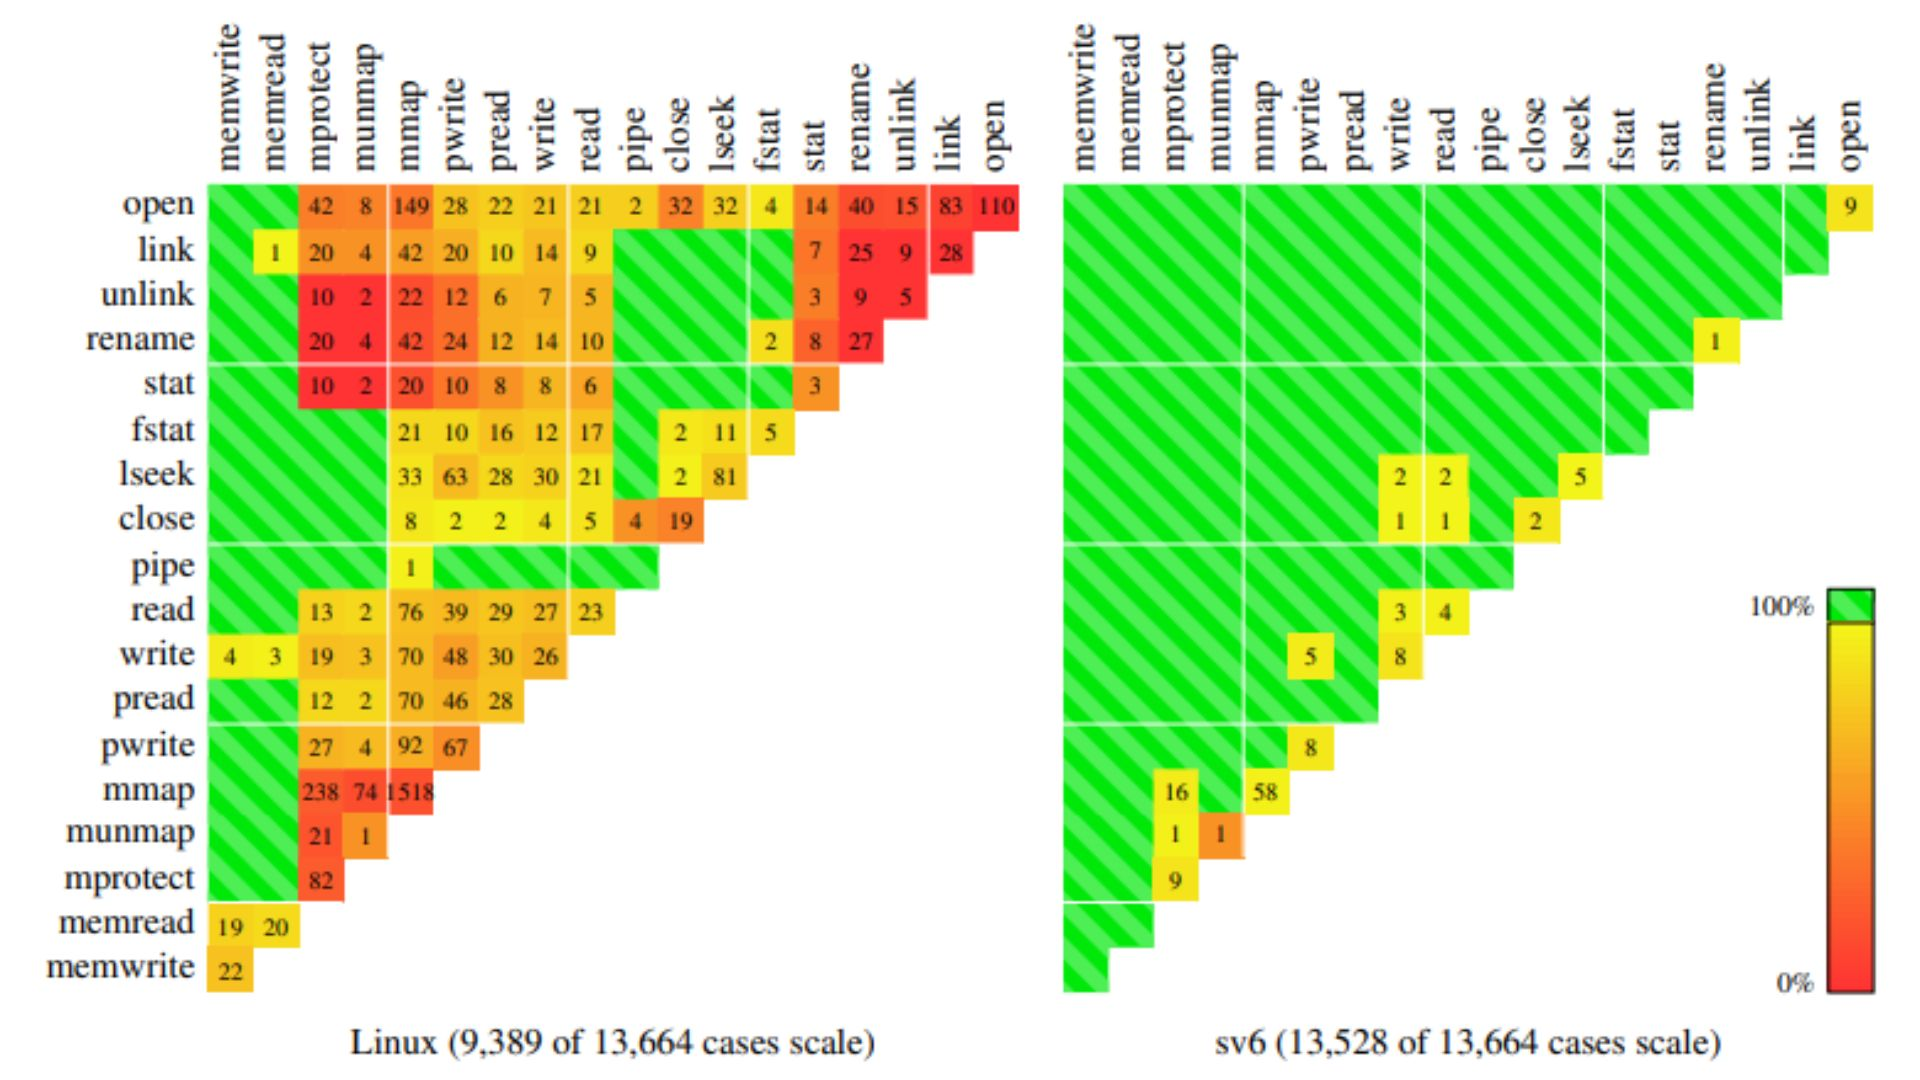
\includegraphics[width=0.5\textwidth]{Images/Paper44Figure.jpg}
    \caption{Image from the Paper: The Scalable Commutativity Rule: Designing Scalable Software for Multicore Processors}
\end{figure}


\section{DP-SLAM: Fast, Robust Simultaneous Localization and Mapping Without Predetermined Landmarks (68)}

\begin{enumerate}
    \item \textit{Category:} The paper tells of a development in simultaneous localization and mapping (SLAM)
    for robots that can move. Specifically, the paperfocuses on presenting Distributed ParticleSLAM (DP-SLAM), utilizing relevant developments such as the EM and FastSLAM
    algorithms.
    
    \item \textit{Context:} The paper mentions the EM and FastSLAM algorithms as references used in the
    development of DP-SLAM. Burgard was cited to note that various approaches to the EM
    algorithm served to partially separate the localization components from the mapping
    componentsof SLAM.On the other hand, Murphy was mentioned to indicate the relevance
    of the FastSLAM algorithm, providing conditional independences that were integrated into
    DP-SLAM.

    W. Burgard, D. Fox, H. Jans, C. Matenar, and S. Thrun. Sonar-based mapping with mobile
    robots using EM. In Proc. of the International Conference on Machine Learning, 1999.

    K. Murphy. Bayesian map learning in dynamic environments. In Advances in Neural
    Information Processing Systems 11. MIT Press, 1999.
    
    \item \textit{Correctness:} The researchers’assumptions seem to be valid as they have presented empirical results as
    well as multiple figures that resulted from testing their algorithm. DP-SLAM provided more
    accuracy and higher detail in the generated map compared to SLAM.

    \item \textit{Contributions:} The paper’s main contributionis the DP-SLAM algorithm, which entails mapping with higher
    accuracy without the use of predetermined landmarks. The researchers note that this is the
    first time that they know of which achieved thislevel of accuracy considering that they used
    an algorithm that neither closes loops nor has any specific knowledge of the domain.

    \item \textit{Clarity:} The paper is well written: the researchers were able to present their findings well,
    discussing necessary theoretical information and displaying relevant figures whilst taking
    note of the limitations and complexities of their project. They have also stated a point to
    consider for further developments of the algorithm.

\end{enumerate}

\begin{figure}[hb]
    \centering
    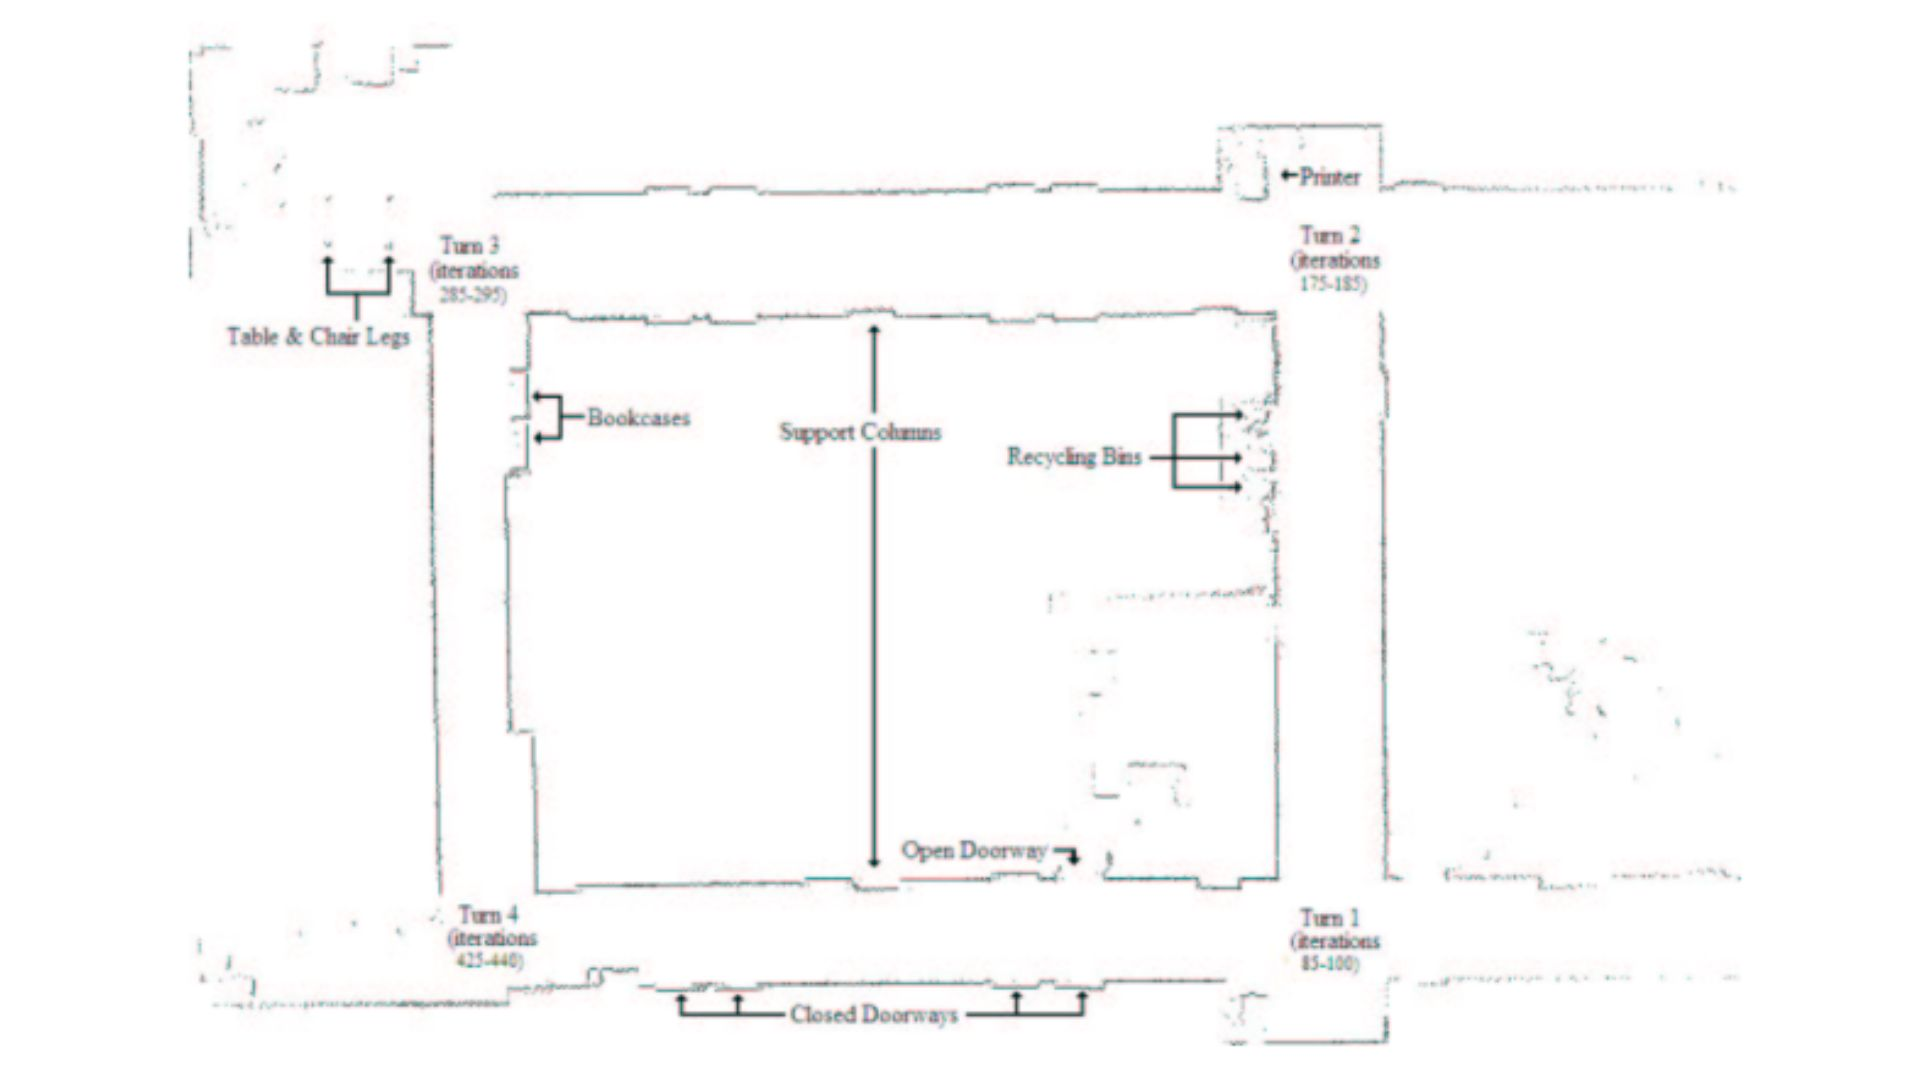
\includegraphics[width=1\textwidth]{Images/Paper68Figure.jpg}
    \caption{Image from the Paper: DP-SLAM: Fast, Robust Simultaneous Localization and Mapping Without Predetermined Landmarks}
\end{figure}


\end{document}